\documentclass[preprint,12pt]{elsarticle}
\usepackage[T1]{fontenc}
\usepackage{lmodern}
\usepackage{amsmath,amssymb,booktabs,array,graphicx,microtype}
\usepackage[hidelinks]{hyperref}
\usepackage{placeins}
\journal{Neurocomputing}
\makeatletter
\let\ps@pprintTitle\ps@plain
\makeatother
\newcommand{\cov}{\operatorname{cov}}
\newcommand{\full}{\operatorname{full}}
\begin{document}
\begin{frontmatter}
\title{From Set Prediction to Evidence Selection: An Empirical Study of Surrogate Objectives in Multi-hop RAG}
\begin{abstract}
Selecting evidence for multi-hop question answering requires a model to rank feasible paragraph sets, not merely recognize annotated support in supplied examples. We study how support-supervised neural set scores transfer across constructed-set prediction, budgeted search, and reader answers. Using shared dense candidates from development paragraph corpora derived from HotpotQA and MuSiQue, we compare first-, second-, and fourth-order factorized scorers with a DeepSets control. A two-round search-aligned continuation trains all models on a common pool of final sets and partial frontiers; an equal-update replay control distinguishes this intervention from additional static training. High constructed-pair accuracy does not ensure stronger selection: the static fourth-order model retains complete annotated support on 70.9\% of HotpotQA development questions, compared with 82.1\% for a feasible six-paragraph dense reference. On a shared 128-question answer panel, continuation changes its complete-support count from 55 to 57 while answer F1 falls from 0.4181 to 0.3766. Same-question analysis locates most of this net decline among questions whose complete-support status remains positive, rather than those gaining support. Second-order continuation instead gives small F1 increases under both examined seeds. Exact ball indexes preserve flat-search choices but increase measured selection time at 128 candidates. These development findings identify distinct decision, answer, and runtime gaps: useful supervision must be assessed through the choices it induces, with simple selectors, actual reader outputs, and complete execution costs retained as separate endpoints.
\end{abstract}
\begin{keyword}
Retrieval-augmented generation \sep Neural set selection \sep Surrogate objectives \sep Multi-hop question answering \sep Search-aligned learning \sep Empirical evaluation
\end{keyword}
\end{frontmatter}

\section{Introduction}
A neural evidence selector can correctly distinguish a supplied complete set from an incomplete alternative and still choose an incomplete set when asked to search. Even when the selected set recovers more annotated support, a reader may produce a worse answer. These are different decisions: predicting a property of a given set, optimizing the prediction over candidate combinations, and using the resulting text to answer a question. For multi-hop retrieval-augmented generation (RAG), a practical selector must succeed along this entire chain while respecting input and computation budgets.

Set selection is an established alternative to independent relevance ranking. SetR treats context construction as a set decision~\cite{lee2025setr}, and RECOMP studies compression and selective augmentation~\cite{xu2024recomp}. Evidence-chain retrieval also models interactions between passages~\cite{zhang2024beam,guo2025interchunk}. These approaches motivate a more specific empirical question: when inexpensive neural set scorers are supervised by known support annotations, which of their measured capabilities transfer to the evidence lists and answers they actually produce? Annotation coverage is a useful training signal, but it is neither an exhaustive description of all valid reasoning paths nor the reader's answer objective.

We investigate this question with a shared candidate pool, paragraph renderer, reader, and input ceiling. The scorers differ in their interaction structure: a first-order model (H1), second- and fourth-order factorized models (H2 and H4), and a DeepSets-style control. They use frozen dense embeddings and train on complete, incomplete, replaced, and redundant support sets. We then compare static training with a search-aligned continuation that directly supervises the deployed score on actual final and partial search states. All architectures receive the same merged error pool. The study also compares vectorized flat search with exact granular-ball and k-means indexes in the conditional scoring space.

The empirical contribution has three parts. First, we connect controlled prediction accuracy to actual selection under the same six-paragraph and tokenizer constraints, using a feasible dense reference to expose errors that candidate reachability alone cannot explain. Second, we trace changes in support and answers on the same questions across all four scorers and two seeds. The joint analysis distinguishes gaining support from changing an answer while retaining support; selected source-text cases further separate missing bridges, competing roles, and lexical answer matching. Third, we measure whether exact index pruning reduces actual selection time, rather than treating fewer inner products as a deployment speedup.

The resulting picture is model-dependent. H4 improves complete-support counts after continuation but loses answer F1 under both examined seeds; H2 shows small gains against its own static checkpoint under both seeds. MMR remains a strong simple reference. For H4, most of the net answer decline occurs among questions with complete support in both conditions, and all inspected answers finish before the output limit. Thus neither a single retrieval scalar nor output truncation explains the observed change. The exact indexes preserve the chosen sets but add runtime at the tested candidate scale.

This is an empirical development study, not a new independent confirmation experiment. The answer panel was part of the TUNE pool used for initial static checkpoint selection, and the paragraph corpora share sources across development roles. We make those dependencies explicit in Section~\ref{sec:data}. Our conclusions concern the tested support-supervised selectors and reader; they do not establish that higher-order representations or graph-based RAG are generally ineffective.

\section{Related work}
\subsection{Selecting interacting evidence}
Dense passage retrieval provides a scalable relevance backbone~\cite{karpukhin2020dpr}, while multi-hop retrieval extends the decision beyond a single passage~\cite{xiong2021mdr}. MMR balances relevance and redundancy~\cite{carbonell1998mmr}; coverage-based summarization provides another established formulation of joint selection~\cite{lin2011submodular}. These are important controls because a structured scorer must justify more than selecting several individually relevant passages.

SetR explicitly shifts RAG from ranking to set selection~\cite{lee2025setr}. RECOMP learns to compress or omit retrieved context~\cite{xu2024recomp}. Beam Retrieval learns multi-hop retrieval through a beam~\cite{zhang2024beam}. Guo et al. build an inter-chunk interaction graph and retrieve evidence chains using semantic and structural relations~\cite{guo2025interchunk}. Our study does not reproduce those systems or compare their published scores across incompatible settings. It examines a smaller family of annotation-supervised scorers, keeping their candidates and answer interface fixed while following the induced decisions.

\subsection{Learning scores that will be optimized}
Higher-order factorization machines use efficient ANOVA computations to model interactions~\cite{blondel2016hofm}; DeepSets provides a permutation-invariant set architecture~\cite{zaheer2017deepsets}. We adopt these established building blocks as controlled model families. Neither polynomial interactions nor permutation invariance alone establishes that a learned score preserves the desired ordering among searched sets.

Training on states encountered during search has a long history. Beam-search optimization incorporates beam errors in sequence learning~\cite{wiseman2016bso}, while conservative objective models address exploitation of learned objectives in offline optimization~\cite{trabucco2021com}. Our continuation applies direct preferences to saved final sets and partial frontiers, using known support rather than answer reward. It jointly changes the training examples, ranking loss, and checkpoint criterion. The comparison therefore evaluates that intervention as a whole, not the isolated causal effect of a particular loss term.

RAG-LER uses language-model supervision and confidence weighting to regulate a reranker~\cite{zhai2025ragler}. Its supervisory object differs from our mapped support annotations. This distinction matters when interpreting failure: a support scorer need not represent reader utility, even if it predicts its annotation target well.

\subsection{Retrieval quality, answer quality, and implementation cost}
Tian et al. distinguish topical relevance from downstream utility using IR relevance judgments~\cite{tian2025relevance}. Their evaluation uses an IR collection and semantic answer measures, whereas ours uses mapped multi-hop supports and saved canonical answer EM/F1. The common issue is the transition from retrieved information to generated output; the label semantics and experimental interventions differ.

An empirical paper can test specific architectural expectations without requiring every component to win. Chen et al.'s analysis of persuasive-dialogue models pairs component comparisons with concrete negative results and error analysis~\cite{chen2021persuasive}. We follow that problem--control--observation organization, without transferring their task-specific explanations to RAG. Finally, center--radius maximum-inner-product bounds are standard search tools~\cite{ram2012tree}. Here a granular ball is an index over conditional scoring vectors, not an independently validated semantic evidence unit. Its value must be assessed by preservation and timing separately.

\section{Study design and models}
\subsection{Evidence units and feasible decisions}
For question $q$, a frozen BGE-large-en-v1.5 encoder~\cite{xiao2023bge} retrieves the top 128 paragraphs $V_q$ from a per-dataset development corpus. Every selector sees this same list. Paragraphs are reconstructed from original sentence sources, with the sentence mapping retained for support evaluation. The selected whole paragraphs, including titles, are rendered in their original BGE order.

Let $T(q,S)$ denote the actual tokenizer length of the complete reader input, including question, protocol, and chat framing. Learned selection uses
\begin{equation}\label{eq:feas}
\mathcal F_q=\{S\subseteq V_q:|S|\leq6,\ T(q,S)\leq1024\}.
\end{equation}
An infeasible paragraph is skipped, not truncated to manufacture a feasible set. Tokenization of the assembled input determines feasibility; standalone paragraph lengths are features, not substitutes for this check. The six-paragraph limit and the 1,024-token ceiling are distinct constraints.

Let $G_q$ denote known supporting annotations and $C(S)$ the annotations recovered through the source mapping. The targets are
\begin{equation}\label{eq:targets}
\cov(S)=\frac{|C(S)\cap G_q|}{|G_q|},\qquad
\full(S)=\mathbf 1[G_q\subseteq C(S)].
\end{equation}
These labels describe annotated support. They do not mark every unannotated paragraph as irrelevant, certify factual truth, or guarantee a correct reader answer. Gold annotations are used to construct FIT supervision and evaluate saved outputs; they are not injected into evaluation candidates or supplied to the deployed scorer.

\subsection{Common neural representation}
For normalized 1,024-dimensional query and paragraph embeddings $e_q,e_i$, we concatenate $e_q,e_i,e_q\odot e_i,|e_q-e_i|$, cosine relevance, and log paragraph length. Scalar features use FIT normalization statistics. A linear transformation, GELU, and layer normalization produce $h_i\in\mathbb R^{128}$, while a query network produces $h_q$ of the same dimension. The features contain no query identifier, target answer, or support-membership flag.

H1, H2, and H4 have full-support and auxiliary coverage heads. For head $t$, the set logit is
\begin{equation}\label{eq:score}
g_{Ht}(S)=b_{qt}(|S|)+\frac{1}{6}\sum_{i\in S}a_{it}
+\sum_{h=2}^{H}\frac{w_{qth}^{\top}E_h(S)}{32\binom{6}{h}},
\end{equation}
where $a_{it}$ is a unary score, $b_{qt}$ is a query-conditioned cardinality bias, and
\begin{equation}
E_h(S)=\sum_{i_1<\cdots<i_h,\ i_j\in S}
v_{i_1}\odot\cdots\odot v_{i_h},\qquad v_i\in\mathbb R^{32}.
\end{equation}
Factors use a linear projection, layer normalization, and $\tanh$. The denominators are fixed at the maximum cardinality six. H1 omits the interaction sum, H2 includes pair interactions, and H4 includes orders two through four. Only the full-support logit $g$ selects sets; the coverage head is auxiliary.

The DeepSets control retains the unary and cardinality terms and adds a two-output MLP applied to $[\sum_{i\in S}h_i/6,h_q]$, with hidden width 192. It has 707,922 parameters, compared with 670,640 for H2 and 687,152 for H4. H1 registers 662,384 parameters, but 4,192 in its unused interaction projection do not affect the score. Its effective scored capacity is 658,192 parameters. The models share inputs and supervision, but this is not an exact parameter-count match.

\subsection{Flat search and feasible baselines}
Vectorized Flat search begins with the empty set. At each of six depths, each retained parent proposes its four highest-scoring feasible distinct extensions; the global beam keeps four unique sets. All visited sets, not only surviving parents, remain eligible for the final decision. A feasible Dense-K6 reference is also included. The final choice maximizes $g$, with fewer actual input tokens and then stable paragraph identities breaking ties. Negative increments do not stop expansion. Exact extension ranking does not make this finite beam globally optimal.

Dense-budget traverses the dense list and accepts each paragraph that still fits. MMR-budget uses $0.7e_q^\top e_i-0.3\max_{j\in S}e_i^\top e_j$, skipping infeasible additions. These two baselines may retain more than six short paragraphs. Dense-K6 and MMR-K6 add the learned selectors' cardinality limit. All methods use the same final BGE-order renderer. Consequently, comparisons with budget baselines are shared-ceiling pipeline comparisons; comparisons with K6 references more closely match selection constraints.

\subsection{Exact indexes and their limited guarantee}
The ANOVA recurrence updates $E_h\leftarrow E_h+v_i\odot E_{h-1}$ in descending order, with $E_0=\mathbf1$~\cite{blondel2016hofm}. For a fixed parent $S$, an H4 extension can be expressed as
\begin{equation}
g(S\cup\{i\})=o_q(S)+\theta_q(S)^\top z_i,
\qquad z_i=[a_i/6,v_i].
\end{equation}
This converts conditional extension ranking into maximum-inner-product search. For a node with center $c_B$ and maximum Euclidean radius $r_B$, the standard bound is
\begin{equation}\label{eq:bound}
\max_{i\in B}\theta^\top z_i\leq\theta^\top c_B+\|\theta\|_2r_B.
\end{equation}
It follows directly from Cauchy--Schwarz and $r_B=\max_i\|z_i-c_B\|_2$. An average radius would not suffice. The granular-ball index partitions by farthest pivots; the k-means index uses iterated two-center assignments. Both retain every paragraph, share the bound and token checks, and preserve ties at the pruning boundary.

This is an implementation-preservation guarantee relative to the same Flat extension ranking, not a new optimization theorem or an answer-quality guarantee. Per-query factor construction, tree building, traversal, and token checks remain real costs. Section~\ref{sec:cost} assesses whether reducing scored candidates compensates for them.

\section{Data, supervision, and interventions}\label{sec:data}
\subsection{Development roles and candidate reachability}
The development material contains 4,000 previously exposed HotpotQA and MuSiQue questions~\cite{yang2018hotpotqa,trivedi2022musique}. The group split yields FIT 3,166, TUNE 738, and historical development 96 (Table~\ref{tab:roles}); FIT contains 3,165 groups. The reconstructed corpora contain 9,791 HotpotQA and 31,130 MuSiQue paragraphs. This is corpus retrieval over the available development material, not full-Wikipedia retrieval. BGE retrieval is exact, without ANN approximation. Its 512-token encoder limit truncates 16 and eight paragraphs, respectively; reader feasibility is checked separately.

\begin{table}[t]\centering\small
\caption{Data roles. MINE is a subset of FIT. DEV-SELECT and QA are disjoint subsets of TUNE, but the entire TUNE pool was used for initial static checkpoint selection.}\label{tab:roles}
\begin{tabular}{@{}p{2.8cm}rrp{5cm}@{}}\toprule
Role & HotpotQA & MuSiQue & Use\\\midrule
FIT & 748 & 2,418 & Supervised training\\
TUNE & 196 & 542 & Initial checkpoint loss; selection analysis\\
Historical development & 56 & 40 & Earlier exposed material\\
MINE & 256 & 256 & Shared search-state training pool\\
DEV-SELECT & 64 & 64 & Continuation checkpoint selection\\
QA & 64 & 64 & Saved reader-answer comparison\\\bottomrule
\end{tabular}\end{table}

Question groups do not cross roles, but FIT and TUNE share 57 HotpotQA and 4,753 MuSiQue source documents. Initial static checkpoints were selected by loss on all TUNE questions, including QA. Only the later continuation criterion uses DEV-SELECT without QA. Thus the QA results are exposed development comparisons, even though answer F1 itself did not select continuation checkpoints. QA includes 48 HotpotQA bridge and 16 comparison questions, and 32 two-hop and 32 longer-hop MuSiQue questions. Repeated models and seeds reuse these same 128 questions.

On TUNE, Top128 contains complete known support for 190/196 HotpotQA and 367/542 MuSiQue questions. Considering the original support paragraphs separately, known support fits the input and cardinality limits for 196/196 and 533/542. Reachability and feasibility are different bottlenecks: a support set may fit but not be retrieved. All questions, including nine budget-infeasible MuSiQue cases, remain in the unconditional results.

\subsection{Static supervised sets}
Static FIT supervision includes complete known-support sets, missing-support sets, same-size replacements, redundant additions, Dense-K6/MMR-K6, and limited random examples. FIT reference construction can append missing support paragraphs and matched distractors to create training sets. This training operation is not used by evaluation or search-state mining, which retain the original Top128.

The base loss combines full-support binary cross-entropy, $0.5$ times sigmoid coverage MSE, $0.25$ times pointwise annotation classification, and $0.25$ times a softplus preference for constructed complete/incomplete pairs of equal cardinality. AdamW uses learning rate $10^{-3}$ and weight decay $10^{-4}$. The initial study retained seeds 1729, 2026, and 426; the continuation comparison uses 1729 and 2026. The third static seed is retained in the numerical supplement but is not relabeled as a continuation run.

Constructed-pair accuracy tests a supplied pair distribution. Actual selection tests an optimized distribution of sets, including combinations never represented by those particular pairs. We therefore report pair accuracy, selected support, reader answers, and cost as distinct endpoints. The same-size training control limits an obvious cardinality shortcut but does not eliminate all length or distribution effects.

\subsection{Shared search-aligned continuation}
MINE contains 512 FIT questions selected by deterministic group hash, balanced across datasets with existing question-type strata retained. Each model searches with its current score. A shared pool merges final sets, high-scoring partial frontiers, Dense-K6/MMR-K6, and at most eight deterministic feasible replacement attempts per trajectory. The deduplicated pool is capped at 64 sets per question, prioritizing model finals and high-scoring frontiers. All four models train on the same pool; no model receives exclusive candidates, stronger supervision, or a different reader.

For the annotation utility $u(S)=[\full(S)+\cov(S)]/2$, a preferred pair has $u(S^+)>u(S^-)$. The added loss directly supervises the deployed logit:
\begin{equation}\label{eq:pref}
\ell(S^+,S^-)=\log\left(1+\exp\left\{0.2[u(S^+)-u(S^-)]-[g(S^+)-g(S^-)]\right\}\right).
\end{equation}
Final-set pairs prefer equal cardinality and token ratios within $[0.8,1.25]$, falling back to equal cardinality. Frontier pairs prefer a shared parent and depth, with same-depth fallback. Missing pair categories are masked rather than fabricated. Importantly, partial sets with zero full labels can still receive different preferences through coverage, and those preferences affect $g$, not merely the auxiliary head.

The continuation loss is $L_{\rm base}+0.5L_{\rm final}+0.5L_{\rm frontier}$. Each query supplies four static and four mined base observations and up to one pair per added category. Losses are normalized within and across queries. Each of at most two rounds permits eight epochs, using AdamW at $3\times10^{-4}$, weight decay $10^{-4}$, query batch eight, and gradient clipping at one. A second round re-mines the selected current models.

Not every query supplies a preference. For primary-seed round one, final pairs are unavailable for 171/256 HotpotQA and 115/256 MuSiQue questions; frontier pairs are unavailable for 17 and 42. The corresponding round-two counts are 196/135 and 19/59. Every question still supplies base supervision. These counts limit the interpretation of the intervention: a large pool does not necessarily yield informative pairwise gradients for every query.

\subsection{Checkpoint and replay controls}
At epochs two, four, and eight, continuation checkpoints are compared by dataset-equal complete support on DEV-SELECT, then coverage, lower original loss, and earlier checkpoint. Every selected model comes from the first round. No QA-answer score is used for this decision. H4 replay uses eight static sets per query and the same number of optimizer updates as the selected aligned H4 checkpoint. It controls extra updates, not all computation, since added pair terms require additional evaluations. The intervention changes examples, preferences, and checkpoint selection together; it is not a pure loss ablation.

\subsection{Reader, outcomes, and new descriptive analyses}
The reader is the original FP16 Qwen2.5-3B-Instruct~\cite{qwen2024release}, with greedy decoding, at most 128 output tokens, and the shared P2 single-answer-field protocol. It uses no relation-front-end adapter. Identical model, input tokens, precision, decoding, and protocol identities permit cached output reuse; cache reuse is not independent generation. Existing canonical EM and token F1, including dataset-specific answer handling, are reused without rescoring or answer cleanup. Format failures remain in the denominator.

The new analyses are post hoc descriptions of these completed runs. We form pairs by question, dataset, model, seed, budget, and protocol. Full-support transitions are $00,01,10,11$. F1 changes above $10^{-12}$ or below $-10^{-12}$ define increase or decrease; the tolerance only handles floating-point differences. For transition group $A$, its contribution to the observed panel mean is
\begin{equation}\label{eq:decomp}
d_A=\frac{1}{N}\sum_{i\in A}(F1_{i,\rm aligned}-F1_{i,\rm static}),\qquad N=128.
\end{equation}
This is an additive descriptive decomposition, not a causal attribution. All four models and both seeds are retained, with per-dataset tables in the supplement. No new bootstrap, hypothesis test, or significance claim is introduced.

We also inspect saved selection logits in fixed sigmoid bins $[0,.2,\ldots,1]$, reporting counts and annotated completeness, including empty bins. These are search-selected TUNE outputs, not an independent probability-calibration sample. Finally, 16 distinct H4 questions are selected by a fixed hash within dataset, support-transition, and F1-direction cells: primary-seed gain/harm cells first, then new questions from the second seed, with unchanged cells only if needed. Question and source text are read before saved answers. This assistant-assisted case review is not independent expert annotation and estimates no population error rate.

\section{Results}
\subsection{RQ1: Does supplied-set prediction transfer to selection?}
Constructed complete/incomplete pair accuracy is high under the primary seed. H4 achieves 0.9645 on HotpotQA and 0.9464 on MuSiQue; H2 achieves 0.9638/0.9422 and DeepSets 0.9620/0.9482. H1 is lower at 0.9475/0.8978. These values show that the supplied training-style distinction is learnable, but do not establish that H4 ranks the alternatives encountered in search better than its controls.

\begin{table}[t]
\centering\small
\caption{Annotation gap to the feasible Dense-K6 reference on all TUNE questions, static H4, seed 1729. Loss/gain counts are relative to that reference. These are retained aggregate diagnostics; per-query reference logits were not saved.}\label{tab:reference}
\begin{tabular}{lrrrrr}\toprule
Dataset & $N$ & Dense-K6 full & H4 full & Lost & Gained \\
\midrule
HotpotQA & 196 & 0.8214 & 0.7092 & 27 & 5 \\
MuSiQue & 542 & 0.2565 & 0.2232 & 42 & 24 \\
\bottomrule\end{tabular}
\end{table}

The feasible-reference comparison makes that distinction concrete (Table~\ref{tab:reference}). Dense-K6 recovers complete annotated support for 82.1\% of HotpotQA TUNE questions, compared with 70.9\% for static H4. Relative to the reference, H4 loses 27 complete cases and gains five. On MuSiQue it loses 42 and gains 24, with completeness 22.3\% versus 25.6\%. Since Dense-K6 is explicitly eligible for final selection, these errors cannot all be attributed to the beam failing to visit that feasible reference.

The retained diagnostic reports no selected H4 score below its Dense-K6 reference (tolerance $10^{-8}$). However, only aggregate score differences and transition counts were saved; the per-question reference scores and sets were not retained by that diagnostic. We therefore preserve its annotation comparison without manufacturing a new paired logit distribution or claiming global optimization regret. No model was loaded to fill that gap. Missing MMR-K6 paired scores are likewise unavailable.

\begin{figure}[t]\centering
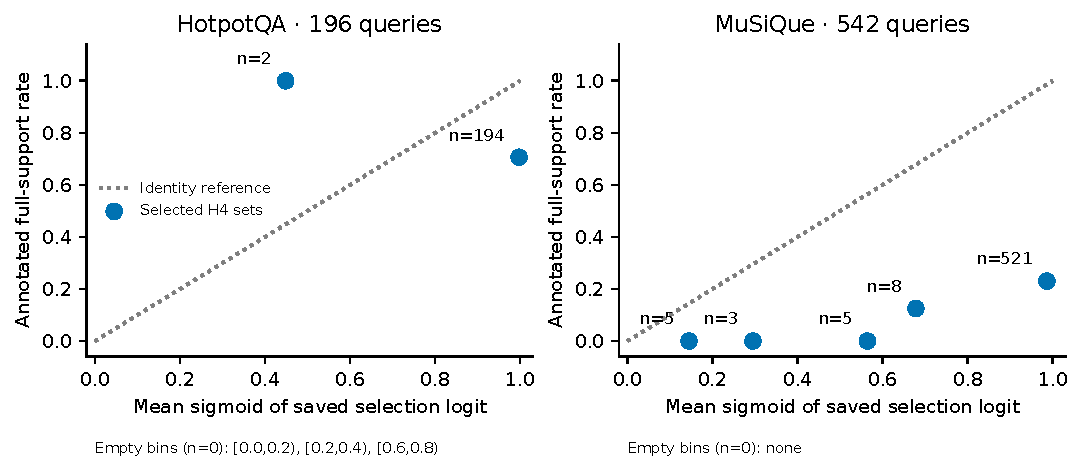
\includegraphics[width=\linewidth]{selected_scores.pdf}
\caption{Saved static H4 outputs after search, seed 1729. Each point summarizes one fixed sigmoid bin; annotations give actual bin counts. The diagonal is an identity reference, not a fitted calibration curve. These selected TUNE sets support a descriptive score--annotation discrepancy, not independent calibration or a paired Dense-K6 score-gap distribution.}\label{fig:scores}
\end{figure}

Figure~\ref{fig:scores} shows the discrepancy among saved selected sets directly. In the highest bin, 194 HotpotQA sets have mean sigmoid output 0.9976 but annotated completeness 0.7062. The corresponding 521 MuSiQue sets have mean 0.9867 and completeness 0.2303. The supplement gives the same bins for all four models. Concentration near one is not unique evidence of a high-order failure: the highest DeepSets bins contain 194 and 539 sets, with completeness 0.6959 and 0.2319. Search-selected outputs should therefore not be interpreted as calibrated probabilities from their numeric range alone.

A separate existing matched-length pair diagnostic also limits the higher-order interpretation. H4 pair accuracy is 0.8333/0.7878, compared with 0.9524/0.8525 for DeepSets, on 84/278 pairs from 65/185 queries. This smaller diagnostic changes the supplied-pair distribution and is not a new QA evaluation. Together, the results support a decision-distribution mismatch in the tested scorers; they do not show that adding interactions universally improves evidence choice.

\subsection{RQ2: What changes after search-aligned training?}
\begin{table}[t]
\centering\small
\caption{Answers and selected contexts on the same 128 development questions (64 per dataset), seed 1729. F1 and EM are proportions. Dense and MMR share the 1,024-token ceiling but may exceed six paragraphs; learned models cannot. Replay matches optimizer steps, not total computation.}\label{tab:qa}
\begin{tabular}{lrrrrr}\toprule
Selector & Full & F1 & EM & Blocks & Input tokens \\
\midrule
Dense & 64/128 & 0.4055 & 0.3359 & 6.95 & 1009.9 \\
MMR & 61/128 & 0.4303 & 0.3672 & 7.25 & 1007.3 \\
H4 static & 55/128 & 0.4181 & 0.3594 & 5.91 & 916.9 \\
H4-replay & 55/128 & 0.4046 & 0.3359 & 5.91 & 900.9 \\
H1 aligned & 61/128 & 0.4065 & 0.3359 & 4.45 & 696.2 \\
H2 aligned & 56/128 & 0.4057 & 0.3516 & 5.53 & 789.7 \\
DeepSets aligned & 60/128 & 0.4090 & 0.3516 & 4.43 & 693.4 \\
H4 aligned & 57/128 & 0.3766 & 0.2969 & 5.70 & 842.2 \\
\bottomrule\end{tabular}
\end{table}

Table~\ref{tab:qa} retains simple selectors, the static H4 checkpoint, replay, and all aligned models on the same answer panel. MMR has answer F1 0.4303, compared with 0.4181 for static H4 and 0.3766 for aligned H4. H4's complete-support count rises from 55 to 57, but EM falls from 0.3594 to 0.2969. Replay gives F1 0.4046 with 55 complete-support questions. Additional static updates therefore do not reproduce the aligned endpoint, although equal updates are not equal total compute.

The contexts differ in realized size. Dense and MMR average 6.95 and 7.25 paragraphs and about 1,010 and 1,007 input tokens. Static and aligned H4 average 5.91 and 5.70 paragraphs and 917 and 842 tokens. This is a meaningful shared-ceiling comparison but not a context-length-matched answer experiment. Shorter aligned input may reduce reader work, yet the intervention did not isolate length from content. Its F1 change cannot be attributed to shortening alone.

\begin{table}[t]
\centering\small
\caption{Each aligned model against its own static checkpoint on the same QA panel. The seeds reuse the same 128 questions; they do not create independent samples.}\label{tab:paired}
\begin{tabular}{llrrrr}\toprule
Seed & Model & Full count & Static F1 & Aligned F1 & $\Delta$F1 \\
\midrule
1729 & H1 & 50 $\to$ 61 & 0.3738 & 0.4065 & +0.0326 \\
1729 & H2 & 47 $\to$ 56 & 0.3998 & 0.4057 & +0.0060 \\
1729 & H4 & 55 $\to$ 57 & 0.4181 & 0.3766 & -0.0415 \\
1729 & DeepSets & 54 $\to$ 60 & 0.4123 & 0.4090 & -0.0033 \\
2026 & H1 & 49 $\to$ 56 & 0.4277 & 0.4126 & -0.0151 \\
2026 & H2 & 53 $\to$ 54 & 0.4123 & 0.4173 & +0.0051 \\
2026 & H4 & 53 $\to$ 57 & 0.4304 & 0.3831 & -0.0473 \\
2026 & DeepSets & 45 $\to$ 56 & 0.4027 & 0.3521 & -0.0505 \\
\bottomrule\end{tabular}
\end{table}

The own-static comparisons in Table~\ref{tab:paired} prevent an overbroad negative conclusion. H2 gains 0.0060 and 0.0051 F1 under seeds 1729 and 2026. H1 gains 0.0326 under the first seed but loses 0.0151 under the second. DeepSets and H4 lose F1 under both, despite increased complete-support counts. For second-seed H4, full support changes from 53 to 57 and F1 from 0.4304 to 0.3831. These are descriptive development differences, not evidence of statistical equivalence, significance, or guaranteed future performance.

\subsubsection{Joint support--answer transitions}
\begin{figure}[t]\centering
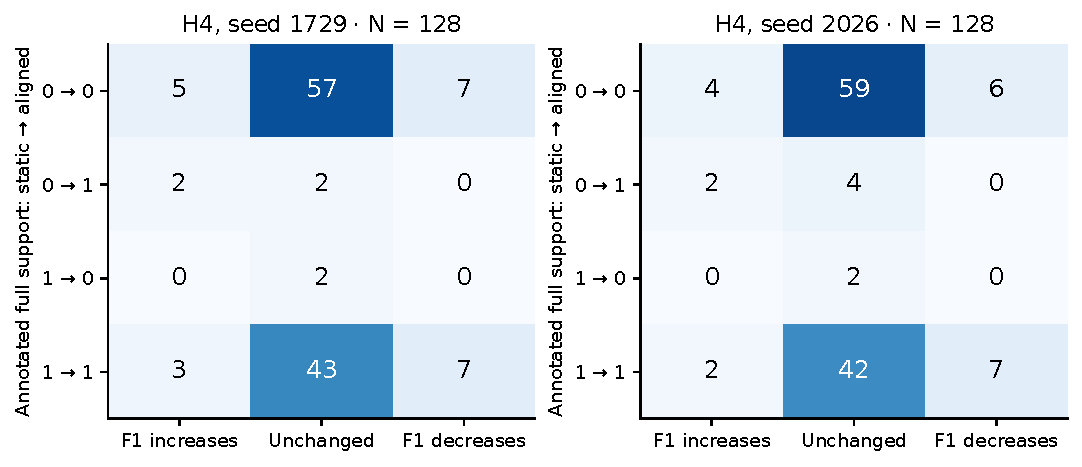
\includegraphics[width=\linewidth]{joint_transitions.pdf}
\caption{Same-question joint transitions for H4. Each panel contains all 128 questions, not only changed or successful cases. The two seeds reuse the same questions. Cells are reconstructed from actual paired records, rather than inferred from separate support and F1 margins.}\label{fig:joint}
\end{figure}
Under the primary seed, full support improves for four questions and worsens for two; 122 retain their status. F1 improves for ten, worsens for 14, and remains unchanged for 104. Those margins alone cannot identify which support changes accompany answer changes. Figure~\ref{fig:joint} and Table~\ref{tab:decomp} use their actual intersection.

\begin{table}[t]
\centering\small
\caption{Descriptive decomposition of H4 answer change. The last column is the group sum divided by all 128 questions, so its four entries sum to the panel difference. It is not a causal attribution.}\label{tab:decomp}
\begin{tabular}{lcrrrr}\toprule
Seed & Full transition & $n$ & $\sum\Delta$F1 & Group mean & Panel contribution \\
\midrule
1729 & 0 $\to$ 0 & 69 & -2.8810 & -0.0418 & -0.0225 \\
1729 & 0 $\to$ 1 & 4 & +1.6667 & +0.4167 & +0.0130 \\
1729 & 1 $\to$ 0 & 2 & +0.0000 & +0.0000 & +0.0000 \\
1729 & 1 $\to$ 1 & 53 & -4.1000 & -0.0774 & -0.0320 \\
2026 & 0 $\to$ 0 & 69 & -1.1190 & -0.0162 & -0.0087 \\
2026 & 0 $\to$ 1 & 6 & +1.1667 & +0.1944 & +0.0091 \\
2026 & 1 $\to$ 0 & 2 & +0.0000 & +0.0000 & +0.0000 \\
2026 & 1 $\to$ 1 & 51 & -6.1000 & -0.1196 & -0.0477 \\
\bottomrule\end{tabular}
\end{table}

The primary-seed $01$ group contributes $+0.0130$ F1 to the whole-panel mean. The $10$ group contributes zero, while $00$ contributes $-0.0225$ and $11$ contributes $-0.0320$, summing to $-0.0415$. Under the second seed, $01$ contributes $+0.0091$, $10$ again zero, $00$ $-0.0087$, and $11$ $-0.0477$, summing to $-0.0473$. Thus the largest net negative component in both runs lies among questions that preserve complete annotated support. It would be incorrect to describe these observations as evidence that newly adding complete support causes harm.

Full-support status is binary and intentionally coarse. Within $11$, the selected surrounding paragraphs, wording, ordering under the common renderer, and actual token lengths can still change. Within $00$, partial coverage can change even though completeness remains zero. The decomposition locates changes; it does not identify an internal attention mechanism or establish which context modification caused an answer to change. The numerical supplement retains coverage, EM, paragraph-count, token-count, and context-identity differences for every pair.

\subsubsection{What the source-text cases clarify}
The selected 16 cases were read in full using retained, removed, and added paragraphs before consulting saved predictions. Four illustrate different limits of the aggregate metrics. An added team paragraph supplies the missing conference bridge in C03; support changes $0\to1$ and F1 rises from 0 to 0.6667, while EM remains zero. C12 adds a company-location paragraph tied to the precise role in the question; support changes $0\to1$ and F1 rises from 0 to 1. These are concrete instances in which a recovered bridge accompanies an improved answer.

C10 retains the creator identity and production-date range in both contexts, but the answer changes from the requested production endpoint to a later rights-transfer year in the same source. Full support remains one while F1 drops from one to zero. The text supports a role/date-selection error description, not a claim about why the reader attended to one date. C11 retains a sponsor's full name and acronym; the output switches from the full name to the acronym, with saved canonical F1 changing from one to zero. That lexical change is not equivalent to losing the named entity from the evidence. We retain the original score and do not introduce a favorable alias rule.

All 32 saved outputs for the 16 paired cases reached EOS and none hit the output cap. Output truncation does not explain these inspected changes. Other cases include unresolved entity links and geographic ambiguity; an answer-score increase by itself does not certify a sufficient evidence chain. The de-identified supplement reports every selected case and its uncertainty. Cases illustrate mechanisms compatible with the text; they do not estimate their prevalence across the 128-question panel.

\subsection{RQ3: Does exact pruning improve actual cost?}\label{sec:cost}
The original index check compares two indexes with Flat on 738 TUNE questions: 1,476 final comparisons and 30,956 extension states show no mismatch. A fixed refined-leaf diagnostic uses 32 questions per dataset and again finds no mismatch across 128 final comparisons and 2,688 states. These are preservation checks under the same score and beam. They do not establish a globally optimal set, and no new index run is introduced here.

\begin{figure}[t]\centering
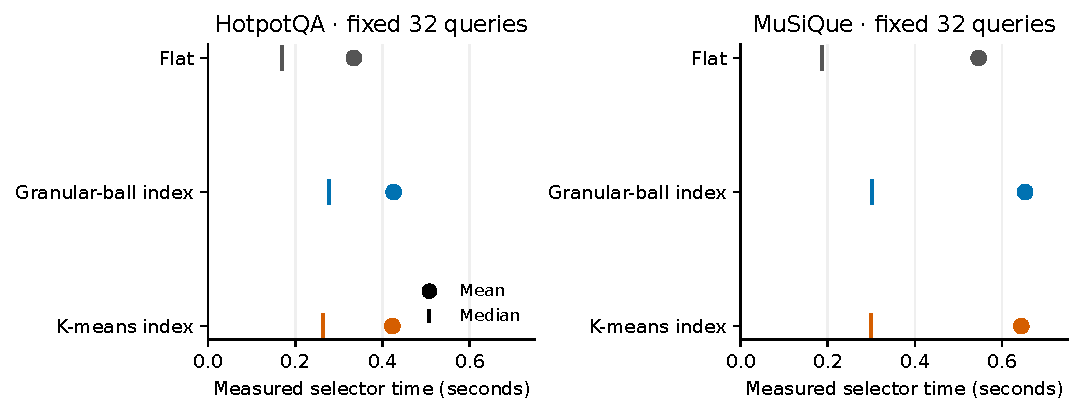
\includegraphics[width=\linewidth]{index_cost.pdf}
\caption{Existing refined-leaf timing diagnostic at 128 candidates, 32 fixed questions per dataset. Dots are means and vertical markers are medians, not confidence intervals. The original per-query timings for this refined subset were not retained; no distributions are invented. Some CPU selection measurements overlapped GPU reader work, so these are implementation measurements rather than isolated hardware benchmarks.}\label{fig:cost}
\end{figure}

At this scale, preservation does not yield a speedup (Figure~\ref{fig:cost}). HotpotQA mean selection time rises from 0.3346 seconds for Flat to 0.4256 for the granular-ball index and 0.4227 for k-means. MuSiQue rises from 0.5461 to 0.6528 and 0.6439 seconds. The granular-ball index reduces mean true extension scores from 2,688 to about 906 and 1,505, respectively, but increases tokenizations from 215 to 281 and from 310 to 383. Traversal order and feasibility work can therefore offset pruning savings. This is an observed cost pattern, not a controlled causal attribution to one component.

Recorded tokenizer time is nested within total selection time; it cannot be stacked on top as an independent cost. Per-query vector and tree construction are included in the measured selector operation, while full process setup and corpus encoding are different accounting scopes. The supplement retains original 738-question timings separately from the refined 64-question aggregates. Results at 128 candidates do not establish how either index scales to a much larger candidate set.

\begin{table}[t]\centering\small
\caption{Recorded execution costs of the two completed studies, including their broader saved panels. These are not the costs of just the 128-question main table. GPU time is model-residency process wall time; CPU is measured process time. Cache hits are logical reuse, not new inference.}\label{tab:cost}
\begin{tabular}{lrr}\toprule
Recorded quantity & Static study & Continuation study\\\midrule
GPU process seconds & 4,350.28 & 4,513.07\\
Measured CPU seconds & 10,541.75 & 7,035.50\\
New reader calls & 2,287 & 986\\
Logical QA rows & 3,520 & 1,536\\
Cache hits & 1,241 & 558\\
Measured generation seconds & 2,532.22 & 867.94\\
Peak allocated GPU GiB & 6.63 & 6.11\\\bottomrule
\end{tabular}\end{table}

Table~\ref{tab:cost} distinguishes actual calls from logical result rows. Each study includes eight reader reruns that bypass the cache, so new calls plus cache hits exceed logical rows by eight. Reusing a prompt does not count as independent generation or an online deployment acceleration. These totals include their original development, sensitivity, and repeat work; they cannot be divided by the main panel size to estimate a single-query serving cost. Earlier unmeasured CPU remains unknown. The present manuscript analysis uses only saved records and introduces no model call, training, answer rescoring, or GPU experiment.

\section{Discussion and limitations}
\subsection{Three gaps, with different remedies}
The first gap is between learning to score supplied sets and using that score for selection. A feasible reference remains available, yet the learned objective may prefer sets with less annotated support. This directs attention to the distribution of optimized states and the alignment of the score, rather than only beam width or candidate reachability. The shared-pool continuation addresses that specific issue, but its outcomes differ by model and seed. More expressive interactions do not establish a reliable advantage in these records.

The second gap is between support selection and answer production. Our new joint analysis sharpens that statement: H4's net losses are dominated by support-preserving questions, while recovered support contributes positively to the mean. Annotated completeness therefore hides changes in surrounding context and reader behavior. The source cases add an evaluation-layer distinction: an entity acronym may preserve meaning while changing canonical lexical overlap, whereas choosing a rights-transfer date instead of a production endpoint is a different error. Neither observation justifies changing the scoring rule after viewing answers.

The third gap is between mathematical pruning and measured runtime. The exact indexes are correct relative to Flat, but correctness and fewer inner products do not offset their implementation overhead here. The practical choice at this candidate count is therefore supported by measured latency, not by an assumption that hierarchical search is faster. A larger-scale index study would be a separate empirical question, not an extrapolation from the current counts.

\subsection{Alternative explanations and study boundaries}
The experiments use one frozen encoder, one reader, and one primary 1,024-token interface. Model family, realized context length, and intervention details interact. H4's shorter aligned inputs and different paragraph membership are not isolated factors. MMR and Dense have the same token ceiling but not the same maximum paragraph count; this limits claims of a pure learned-versus-unlearned architecture comparison. The K6 diagnostic establishes a narrower feasible-reference gap in support, without supplying a new K6 answer experiment.

The data are exposed development material. Initial model selection used a TUNE pool containing QA, and source documents overlap FIT and TUNE. Separating later DEV-SELECT does not erase those dependencies. The two seeds reveal sensitivity on the same questions, not two independent confirmation samples. We retain unconditional denominators and do not use a successful-parse, reachable-only, or support-gaining subset as the main answer result. The descriptive analyses add no inferential status to the earlier records.

Support mappings may omit valid alternative evidence. An incomplete annotation set can accompany a correct answer, and complete annotated support can accompany an incorrect or differently phrased answer. Source-text review helps interpret particular cases but is assistant-assisted, outcome-stratified, and limited to 16 questions. It is neither blinded multi-annotator validation nor proof of factual correctness. Per-query Dense-K6 logits and refined-subset timing distributions are missing; the article explicitly distinguishes retained aggregates from newly reconstructible tables.

The studied learned selectors also differ from the project's earlier static evidence-expansion system. The latter used different units, rules, and readers under closed-candidate boundaries. Its positive, negative, and inconclusive historical results remain intact, but cannot validate the mechanisms of the present neural set scorer. Likewise, these results do not rank external graph or hypergraph systems that were not run under the same conditions.

\subsection{Practical implications}
For support-supervised evidence selection, a useful development report should preserve at least four views: supplied-set discrimination, selected-set support, actual answer scores, and measured selection plus reader cost. A feasible simple reference should remain visible even when a learned score assigns it a lower value. Same-question transitions are more informative than comparing unrelated marginal improvements. Finally, an exact implementation should be evaluated for speed independently of its correctness. These recommendations follow from concrete mismatches in the tested system; they are not a claim that one surrogate, architecture, or index is universally preferable.

\section{Conclusion}
We studied how annotation-supervised neural set prediction translates into evidence selection and answers under a shared dense candidate pool and reader budget. Strong constructed-pair discrimination coexists with an annotation gap to a feasible dense reference. Search-aligned continuation changes the deployed decisions, but support and answer outcomes remain model-dependent: H2 shows small development gains under both seeds, whereas H4 gains complete-support cases while losing answer F1. Joint records locate most of H4's net loss among questions retaining complete support, and source cases expose both reader-selection and lexical-matching issues. Exact ball indexes preserve decisions but increase measured cost at 128 candidates. The contribution is this linked empirical account of where the decision chain succeeds and fails, with its development dependencies and missing records explicit.

\section*{Research transparency and AI assistance}
ChatGPT and Codex assisted with research planning, implementation, debugging, analysis scripts, literature organization, case review, manuscript drafting, and editing. The plots were produced programmatically from saved numeric records using Matplotlib, not generated as synthetic experimental images. The new manuscript analyses only join and summarize completed observations; they do not retrain models, rerun retrieval or generation, rescore answers, or add statistical tests. Assistant-assisted case interpretations are distinguished from the recorded model outputs. Final scientific responsibility and approval remain with the human authors.

\section*{Declaration of generative AI use in manuscript preparation}
During manuscript preparation, ChatGPT and Codex were used to help organize arguments, draft and revise English text, check cross-references, and prepare tables and analysis code. Their broader research uses are disclosed above. This author-review version does not represent a completed declaration that all authors have reviewed and approved the final submission.

\section*{Declaration of competing interests}
The authors declare that they have no known competing financial interests or personal relationships that could have appeared to influence the work reported in this paper.

\section*{Data availability}
The study uses existing HotpotQA and MuSiQue materials. The accompanying numerical supplement contains de-identified saved scores, paired descriptive tables, source-role information, and a standalone reconstruction script. It reproduces numerical summaries without model inference or access to raw benchmark answers. Source texts, source identities, and trained weights are not bundled. Release of broader derived materials remains subject to source licenses and author approval; no public weight release is claimed.

\bibliographystyle{elsarticle-num}
\bibliography{references,additions,nc_references}
\end{document}
